\documentclass[12pt, letterpaper]{article}
%BUILD USING XELATEX.

\usepackage{fullpage} %sane margins
%\usepackage{ulem} %strikeouts?
\usepackage{amsmath} %mathematics
%\usepackage{amssymb} %more maths, but conflicts with SIunits :C
\usepackage{graphicx} %GOOD GRAPHICS
\usepackage{subfig, wrapfig}
\usepackage{SIunits} %units
\usepackage{euler} %whoa! smexy!
%for specifying fonts
%cm-default makes equations not look like shit if euler isn't loaded
\usepackage[cm-default]{fontspec}% provides font selecting commands
\usepackage{xunicode}% provides unicode character macros
\usepackage{xltxtra} % provides some fixes/extras
\setmainfont{Times New Roman}

\title{Measuring Anisotropic Thermal Conductivity of Snow and Other Materials Using Needle Probes}
\author{Joshua Holbrook \\ Rorik Peterson}

\begin{document}

\maketitle

\begin{abstract}
Gonna model anisotropic snow conductivity numerically. Then create an anisotropic snow analog in the lab to test the model predictions with well-characterized materials of know conductivity. The three primary questions that will be answered are: (1) ... (2) ... and (3) ... These will be answered by doing ...
\end{abstract}

\pagebreak

\section{Introduction and Background}

The thermal conductivity of snow is an important property for both local and regional climate models in the arctic. During the long period of the year when snow is present, the snow's thermal behavior plays a critical role in calculating the net energy exchange between the ground and atmosphere. The thermal conductivity itself is highly dependent on the temperature gradients that result from this non-equilibrium energy exchange. Snow metamorphism occurs primarily due to vapor transport within the porous snow structure which is driven by the varying vapor pressure of ice as a function of temperature (Figure 1). Sublimation and deposition occur at varying rates within the depth of snow pack, changing the snow microstructure and therefore its associated thermal conductivity.

\begin{figure}[h]
\centering
\caption{Mechanisms for the Development of Anisotropy in Snow}
\subfloat[][Fresh snowfall is relatively homogenous, hence isotropic.]{\label{fig:snow_a} 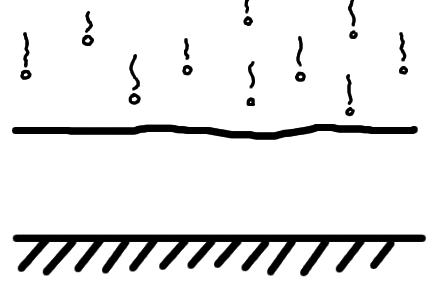
\includegraphics[width=1.6in]{snow_1}}\quad
\subfloat[][Cool air and warm soil cause a temperature differential, with associated difference in vapor pressure.]{\label{fig:snow_b} 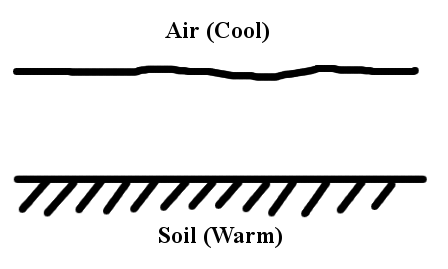
\includegraphics[width=1.6in]{snow_2}}\quad
\subfloat[][Due to these differences in vapor pressure and buoyancy effects, ice sublimes from lower sections of the snow layer and recondenses at regions closer to the surface.]{\label{fig:snow_c} 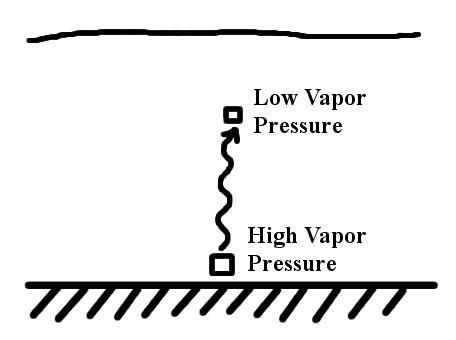
\includegraphics[width=1.6in]{snow_3}} 

\subfloat[][Meanwhile, discrete ice crystals sinter, conglomerating due to diffusion effects (and possibly freeze-thaw events).]{\label{fig:snow_d} 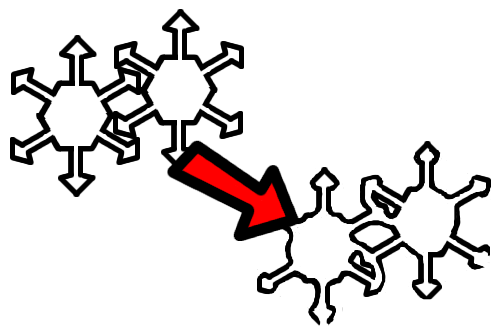
\includegraphics[width=1.6in]{snow_5}}\quad
\subfloat[][The end result is the development of discrete layers in the snow, with more compact snow near the top and less dense snow closer to the ground.]{\label{fig:snow_e} 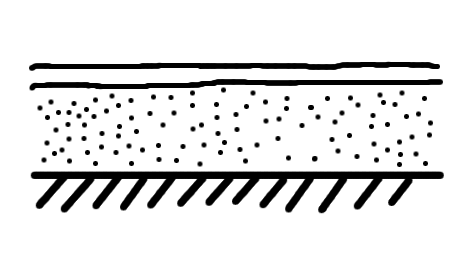
\includegraphics[width=1.6in]{snow_4}}\quad
\subfloat[][Fresh snow adds yet another layer of snow, and the snowscape grows even more complex.]{\label{fig:snow_f} 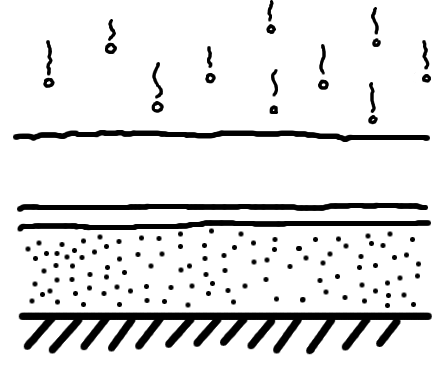
\includegraphics[width=1.6in]{snow_6}}
\label{fig:snow}
\end{figure}

Thermal conduction in porous snow occurs primarily through the solid ice phase and is often limited by the relatively small sintered inter-particle connections. The result of this primarily one-dimensional metamorphism is a layer of low-conductivity material with an anisotropic thermal conductivity. furthermore, this conductivity continues to change with time as the snow surface temperature boundary changes due to both weather and seasonal changes. This thermal-gradient driven anisotropy is further compounded by each subsequent snow event throughout the winter, in which a layer of new snow of relatively low conductivity is deposited on top of older, often more sintered snow.
The importance of quantifying snow thermal conductivity has been recognized for a long time, leading to a number of models based on a range of calculations and observations. Some models are based on the individual particle thermal behavior at the mictrostructural scale, while others on larger-scale laboratory measurements and observed relationships with snow density, temperature, and sometimes age. While the basis for conductivity models can vary widely, there is a slowly growing scientific consensus on the general range of thermal conductivity as a function of snow type or density, although some aspects and details continue to be investigated.
There remains, however, a critical gap between well-characterized thermal conductivity properties of a particular type of snow, and calculating the resulting net energy flux to/from the several layers of anisotropic snow that constitute the natural snowpack. To help bridge this gap, in-situ field measurements of thermal conductivity must be made. The most commonly used device is the needle probe due to the ease with which measurements can be made without substantially disturbing the often fragile snowpack.
The needle probe consists of a very thin, metal rod embedded with a resistive heating element and also a thermistor or thermocouple. The heating element is generates a constant heat flux, and the high conductivity metal guarantees a uniform temperature distribution throughout. The needle is placed into the material and the temperature of the needle measured as a function of time.

\begin{wrapfigure}{L}{0.44\textwidth}
\centering
\label{fig:needle_probe}
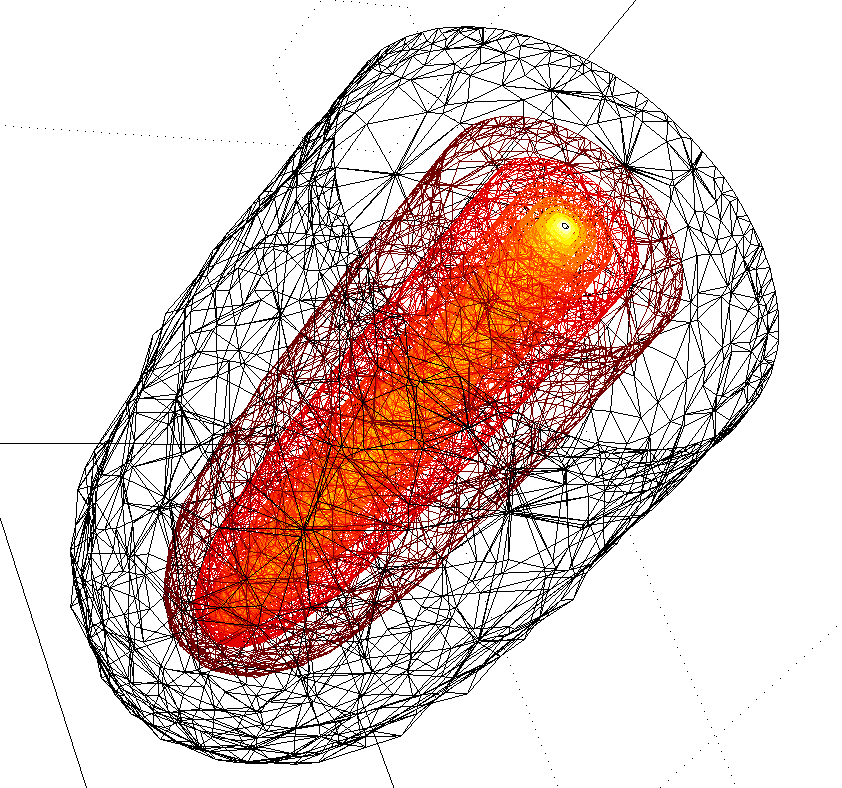
\includegraphics[width=0.4\textwidth]{isotherms}
\caption{A COMSOL model of a needle probe in snow. The surfaces plotted in this visualization represent isotherms in the snow after the needle probe has operated for a "long time."}
\end{wrapfigure}

The thermal conductivity of an isotropic, uniform material surrounding the probe can be determined by approximating the needle as a line energy source, and solving for the temperature as a function of time. The analytic solution to this time-dependent, radially-symmetric problem indicates that the thermal conductivity can be determined by simply plotting the temperature versus natural log of time (\ref{fig:log_graph}).
This technique has appeared to be very successful for measuring the thermal conductivity of many materials including soil, snow, and even food products, and commercial needle probe sensors are widely available. Corroborating measurements using the alternative guarded hot plate method indicate that both techniques are accurate for isotropic materials with uniform properties. However, the viability of the two techniques diverges when attempting to measure anisotropic materials.

\begin{wrapfigure}{R}{0.42\textwidth}
\centering
\label{fig:log_graph}
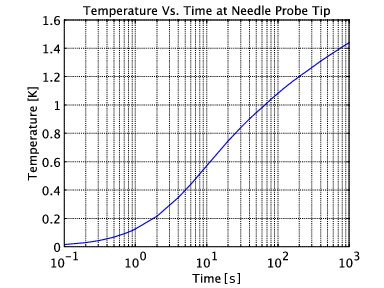
\includegraphics[width=0.4\textwidth]{lolg_scale}
\caption{When plotting \(T\) vs. \(\ln(t)\) of a needle probe, the slope of the linear steady-state portion may be used to calculate the heat conductivity of an isotropic medium.}
\end{wrapfigure}

Because the guarded hot-plate imposes a one-dimensional temperature gradient in rectangular coordinates, it has commonly believed to be the only device of the two that can measure thermal conductivity of anisotropic materials, and then only under prescribed conditions. These necessary conditions require anisotropy in one direction only, and the direction must be known apriori so the sample can be properly oriented in the device.
There therefore exists today a difficulty in measuring the thermal conductivity of an anisotropic snowpack because samples must be carefully extracted from their location, transported in tact to the lab, and properly placed into the guarded hot plate and the conductivity measured. All these steps must be done while not disturbing the sample, or waiting too long between sampling and measurement. Furthermore, the same thermal conditions must be maintained, which may or may not include a thermal gradient, because subsequent metamorphisis may occur. Use of the needle probe would overcome this difficulties because it permits in-situ measurement.

\section{Objectives and Methodology}

The major objectives for this project are three-fold:  First, numerical modeling shall be used to develop a methodology for measuring anisotropic heat conductivity using needle probes. Then, the results will be experimentally corroborated in the laboratory using materials of known, engineered anisotropy. Finally the method will be demonstrated on actual samples of snow.

\subsection{Numerical Modeling}

In the simplest case, and the most familiar one to many, steady-state purely conductive heat transfer is characterized by the following governing equation for one-dimensional heat conduction:

\begin{equation*}
\dot{Q}=-kA\frac{dT}{dx}
\end{equation*}\\

In this case, \(k\) is a scalar property. However, for systems with two or even three dimensions, the governing equation becomes more complex:

\begin{equation*}
\vec{q}=-K \nabla \vec{T}
\end{equation*}

In this equation, \(\vec{q}\) is heat flux (for example, \(\watt \per \square \meter\) ), and \(\nabla \vec{T}\) is temperature gradient. More notable is that instead of a scalar \(k\), this equation has a positive definite matrix \(K\) which encodes anisotropic properties of the material (if the material is in fact isotropic, \(K\) would be a multiple of the identity matrix, making it exactly equivalent to \(k\)).

\begin{wrapfigure}{Rb}{0.42\textwidth}
\centering
\label{fig:m_ellipsoid}
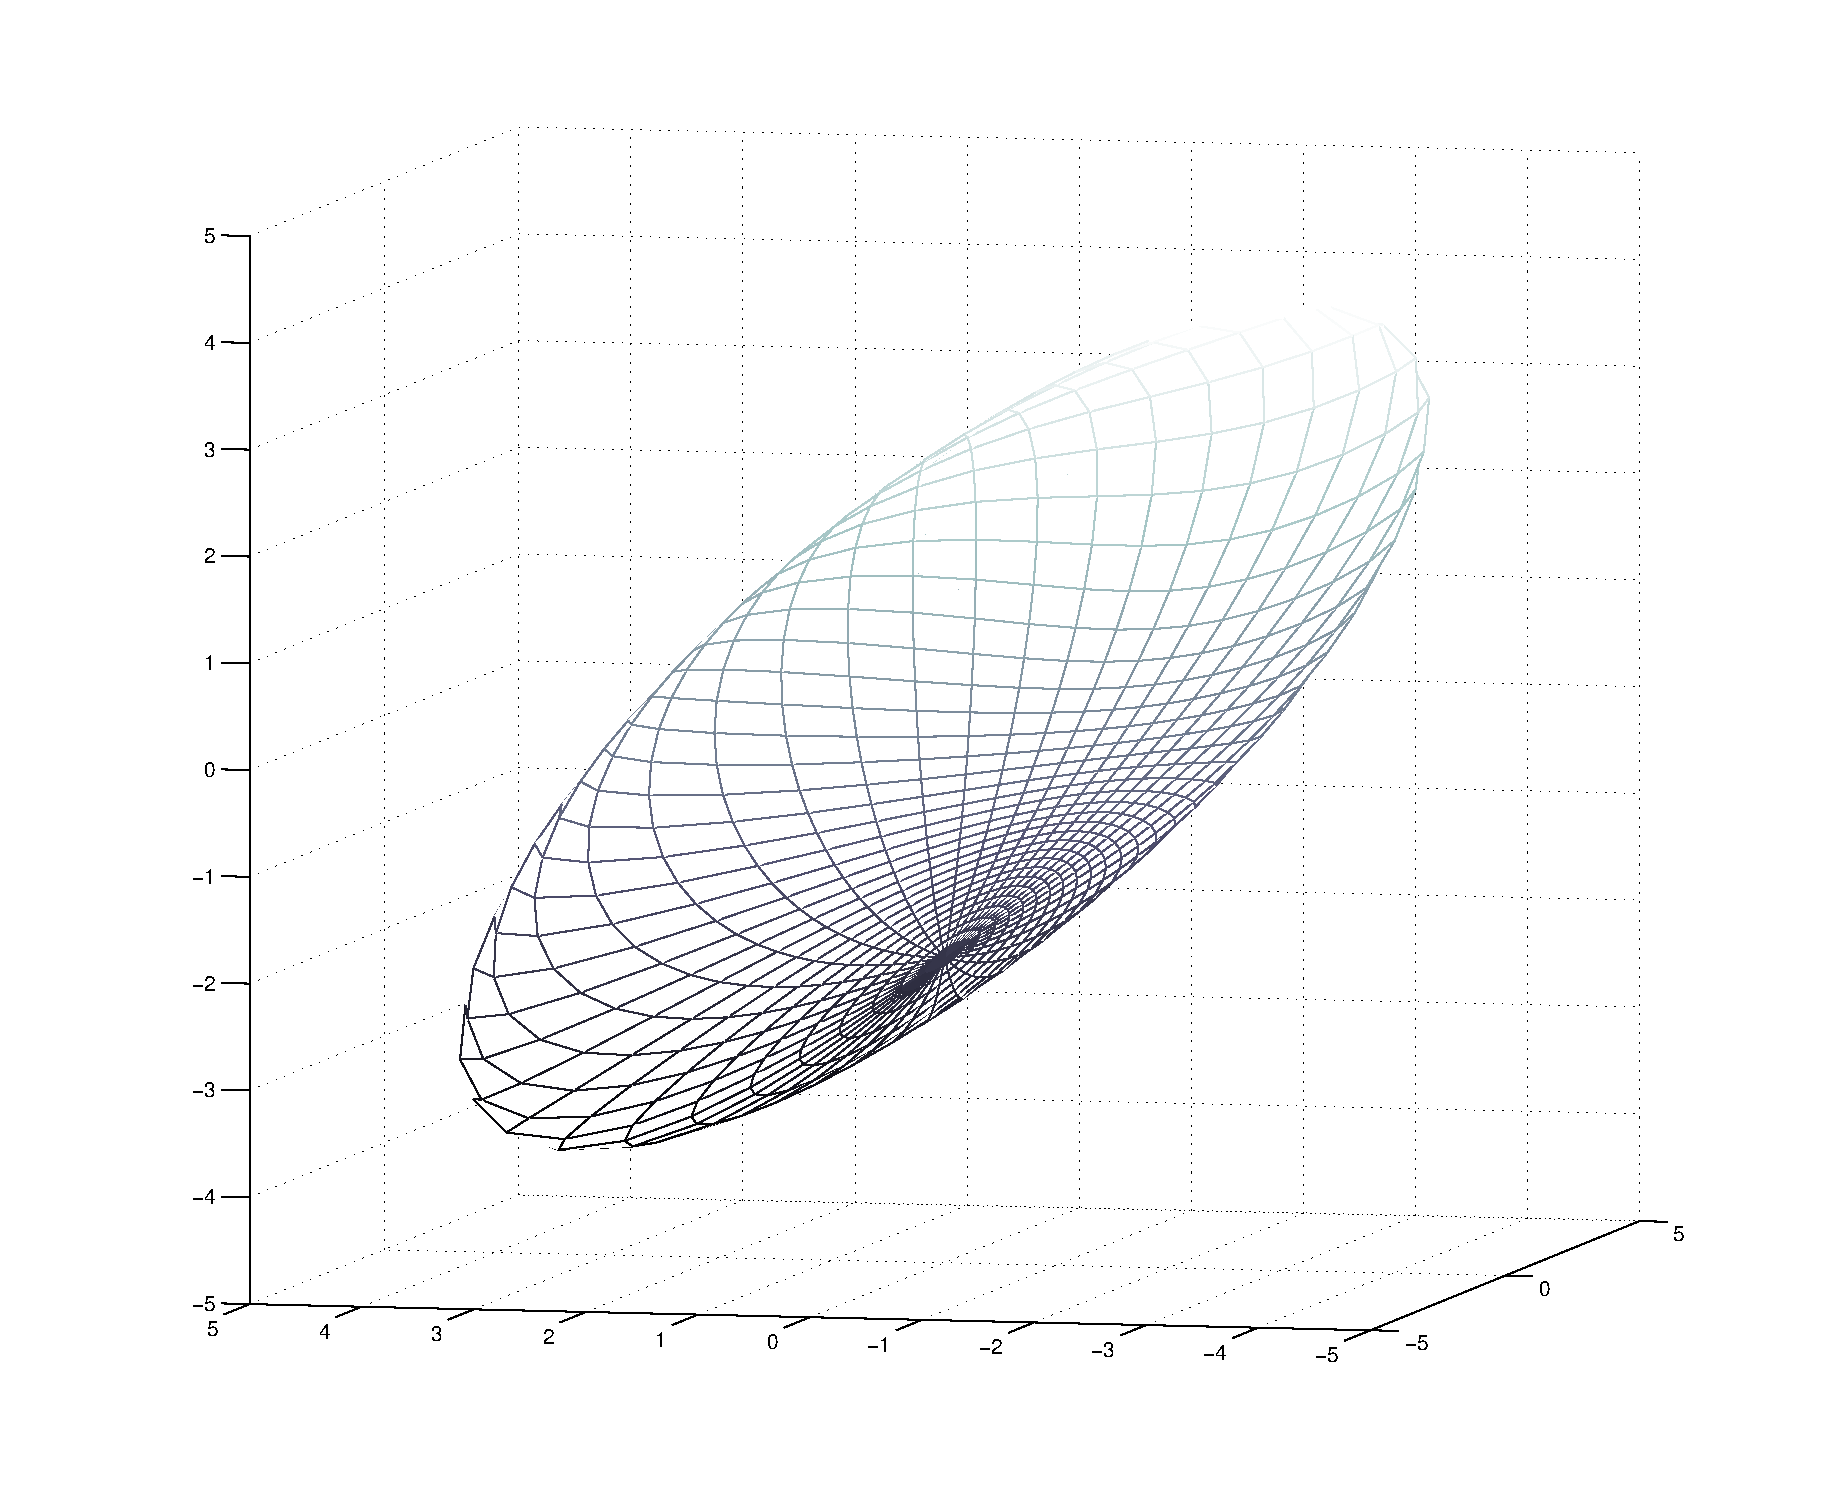
\includegraphics[width=0.4\textwidth]{m_ellipsoid}
\caption{One way to visualize a symmetric, positive-definite matrix such as \(K\) is to plot the ellipsoid \(\vec{x}^TK\vec{x}=1\). The length of a vector \(\vec{x}\) which satisfies this equation is equal to \(1/\sqrt{k}\) for the one-dimensional \(k\) in that direction. Moreover, the semimajor axes of the ellipsoid represent eigenvectors of \(K\). }
\vspace{-72pt}
\end{wrapfigure}

COMSOL and MATLAB will be used to model the behavior of needle probe readings in materials of varying anisotropy and at varying angles with respect to the material's orientation. From this data, we will develop a method for solving for the conductivity matrix of the material based on a minimum amount of measurements.

\subsection{Experimental Corroboration}

Once we have a mathematical model for the material, we will test it in the laboratory. We will assemble composite materials of known anisotropy, made with alternating layers of materials with higher and lower heat conductivity. Examples of considered composites include:
\begin{itemize}
\item Paper and aluminum foil
\item Thin foamboard and ice sheets
\item Thin foamboard and thermal silicone sealant
\end{itemize}
Needle probes will be inserted into these composites and readings will be collected for multiple directions within them. The results from the needle probe method will be compared to results gathered through knowledge of the composite's geometry and guarded hot-plate measurements. This will benchmark the method, allowing us to quantify the associated errors and validate the final numerical model.

\subsection{Field Application Testing}

Finally, once the method is proven in the laboratory, it shall be used in the field to measure the anisotropic thermal conductivity properties of actual snow in the field. Much as will be the case with the artificial composites, needle probe measurements will be taken of snow, from which anisotropy profiles of real snow will be calculated.

\section{References}

TBD

\section{Project Schedule}

TBD

\section{Budget}

TBD

\end{document}
